
%(BEGIN_QUESTION)
% Copyright 2006, Tony R. Kuphaldt, released under the Creative Commons Attribution License (v 1.0)
% This means you may do almost anything with this work of mine, so long as you give me proper credit

Plot the flow rate (Q) of liquid into this vessel, given the graph of liquid volume (V) accumulation over time.  The function you graph (describing liquid flow) will be the {\it time-derivative} of the function shown (describing liquid volume):

$$\includegraphics[width=15.5cm]{i01531x01.eps}$$

\underbar{file i01531}
%(END_QUESTION)





%(BEGIN_ANSWER)

$$\includegraphics[width=15.5cm]{i01531x02.eps}$$

Periods where volume increases linearly (straight-line slope) indicate a constant flow rate into the vessel.  To calculate that flow rate, measure change in volume ($\Delta$V) and divided by change in time ($\Delta$t), for a rise/run slope.

\vskip 10pt

Between 0:00 and 1:00, the volume increased steadily from 0 gallons to 40 gallons over a period of 1 minute.  Therefore, the rate of flow for that time period was 40 gallons per minute.

\vskip 10pt

Between 1:00 and 1:30, the volume remained constant.  This indicates a period of no liquid flow into the vessel, so the flow rate here is 0 gallons per minute.

\vskip 10pt

Between 1:30 and 2:00, the volume increased steadily from 40 gallons to 45 gallons over a period of 0.5 minutes (1/2 minute).  Therefore, the rate of flow for that time period was 10 gallons per minute.

\vskip 10pt

Between 2:00 and 2:15, the volume remained constant.  Again, this indicates a period of no liquid flow into the vessel, so the flow rate here is 0 gallons per minute.

\vskip 10pt

Between 2:15 and 2:45, the volume increased steadily from 45 gallons to 80 gallons over a period of 0.5 minutes (1/2 minute).  Therefore, the rate of flow for that time period was 70 gallons per minute.

\vskip 10pt

Between 2:45 and the end of the graph, the volume remained constant.  No flow into the vessel here (0 gallons per minute).

%(END_ANSWER)





%(BEGIN_NOTES)


%INDEX% Mathematics, calculus: derivative (calculating flow rates from measured volumes at specific times)

%(END_NOTES)


